\subsection{Validazione e collaudo}
Questo periodo inizia il giorno dopo la  \textit{Revisione di Qualifica}(20/04/2019) e si conclude con la consegna dei documenti per la  \textit{Revisione di Accettazione}(10/05/2019). 
\begin{itemize}
	\item{\textbf{Incremento e Verifica:} all’inizio del periodo vengono svolte attività di Incremento e Verifica su vari documenti;}
	\item{\textbf{Glossario:} questa attività comprende sia il miglioramento del Glossario che l’aggiunta dei nuovi termini;}
	\item{\textbf{Validazione e Collaudo:} questa attività consiste nell'attuare vari ed ulteriori test al fine di assicurare la massima qualità conforme agli obiettivi richiesti;}
	\item{\textbf{Manuale Utente:} questa attività consiste nel miglioramento e completamento del \textit{Manuale utente}, contenente indicazioni sull’utilizzo dell’applicazione.}
\end{itemize}

\begin{figure}[h!]
	\centering
	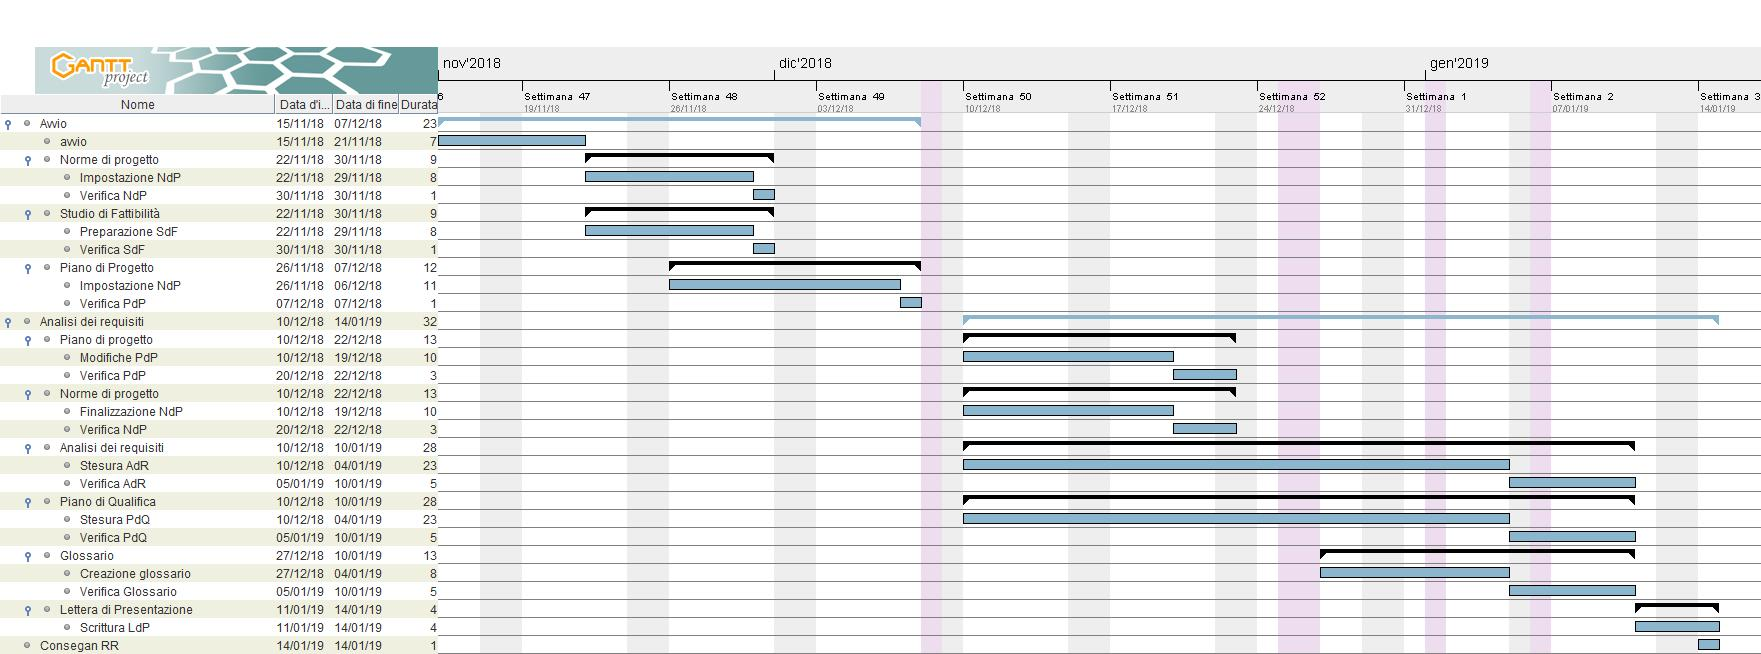
\includegraphics[width=\textwidth]{Gantt_quarta_fase.jpg}
	\caption{Diagramma di Gantt per la fase fino alla Revisione di Accettazione}
\end{figure}

\begin{figure}[h!]
	\centering
	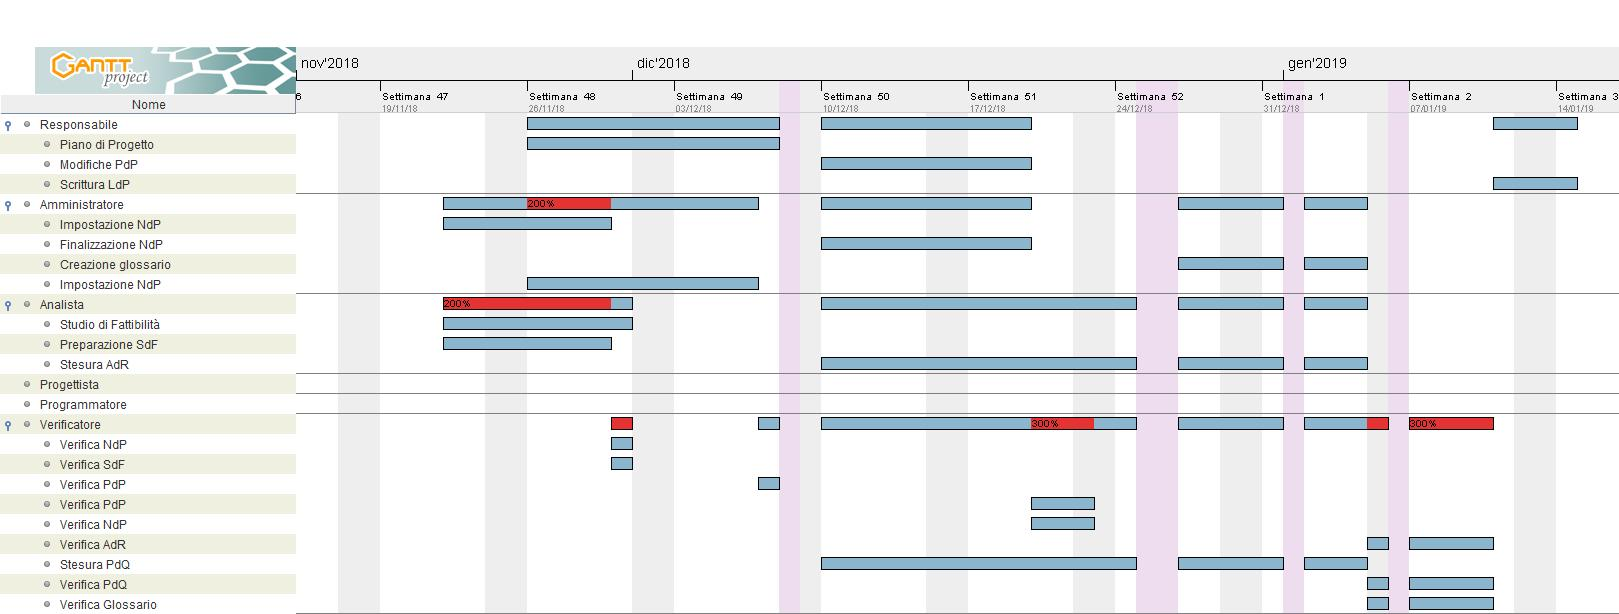
\includegraphics[width=\textwidth]{Gantt_quarta_fase_risorse.jpg}
	\caption{Diagramma di Gantt delle risorse fino alla Revisione di Accettazione}
\end{figure}

\begin{tabular}{|l|l|l|}
	\hline
	\multicolumn{3}{|c|}{\textbf{Suddivisione temporale}}\\
	\hline
	\textbf{Ruolo} & \textbf{20/04/19 - 29/04/19} & \textbf{29/04/19 - 10/05/19} \\
	\hline
	\textbf{Responsabile} & \mat  & \pie   \\
	\hline
	\textbf{Amministratore} & \pie & \mic \\
	\hline
	\textbf{Analista} & \mat \daL \daG & \pie \daG \\
	\hline
	\textbf{Progettista} & - & - \\
	\hline
	\textbf{Programmatore} & \daL \mar & - \\
	\hline
	\textbf{Verificatore} & \mic \daG \gia & \mic \mat \daL \daG \mar \gia \\
	\hline
\end{tabular}